\newpage
\textbf{Tables}
 \begin{table}[ht]
    \caption{Dice Similarity Coefficients (DSC) (mean \pm SD) for prostate, segmented with each of the three trained models (GE, Siemens, and Combined). The results are presented for data from GE and Siemens MRI vendors and the DSCs are calculated on the interpolated (0.5 x 0.5 x 0.5 mm) and original MRI resolution.}
    \begin{tabular}{lcc}
         \hline
          \textbf{Prostate Models} & \textbf{GE (Interpolated/Original Resolution)} & \textbf{Siemens (Interpolated/Original Resolution)}\\
         \hline
         GE & $0.855\pm0.064$/$\mathbf{0.860\pm0.054}$ & $0.804\pm0.099$/$0.802\pm0.106$ \\
         \hline
         Siemens & $0.262\pm0.118$/$0.288\pm0.139$ & $0.892\pm0.038$/$0.889\pm0.035$ \\
         \hline
         Combined & $0.830\pm0.112$/$0.827\pm0.109$ & $\mathbf{0.896\pm0.037}$/$0.892\pm0.036$\\
         \hline
    \end{tabular}
    \label{tab:res_prost}
\end{table} 

\newpage
\begin{table}[ht]
    \caption{Dice Similarity Coefficients (DSC) between manual and CNN-generated PZ contours for GE and Siemens.The trained models are divided in: with (w) data augmentation (DA) and without (wo) DA.}
    \begin{tabular}{lcc}
         \hline
          \textbf{PZ Models} & \textbf{GE Dataset} & \textbf{Siemens Dataset}\\
         \hline
         GE ROI/Original & $0.767\pm0.093$/$0.759\pm0.089$ & $0.537\pm0.204$/$0.539\pm0.204$ \\
         \hline
         Siemens ROI/Original & $0.591\pm0.223$/$0.591\pm0.219$ & $0.808\pm0.085$/$0.808\pm0.087$ \\
         \hline
         Combined ROI/Original & $\mathbf{0.797\pm0.093}$/$0.788\pm0.093$ & $\mathbf{0.813\pm0.079}$/$0.811\pm0.79$\\
         \hline
    \end{tabular}
    \label{tab:res_pz}
\end{table}

\newpage
\textbf{Figure legends:}
\begin{figure}[ht]
    \centering
    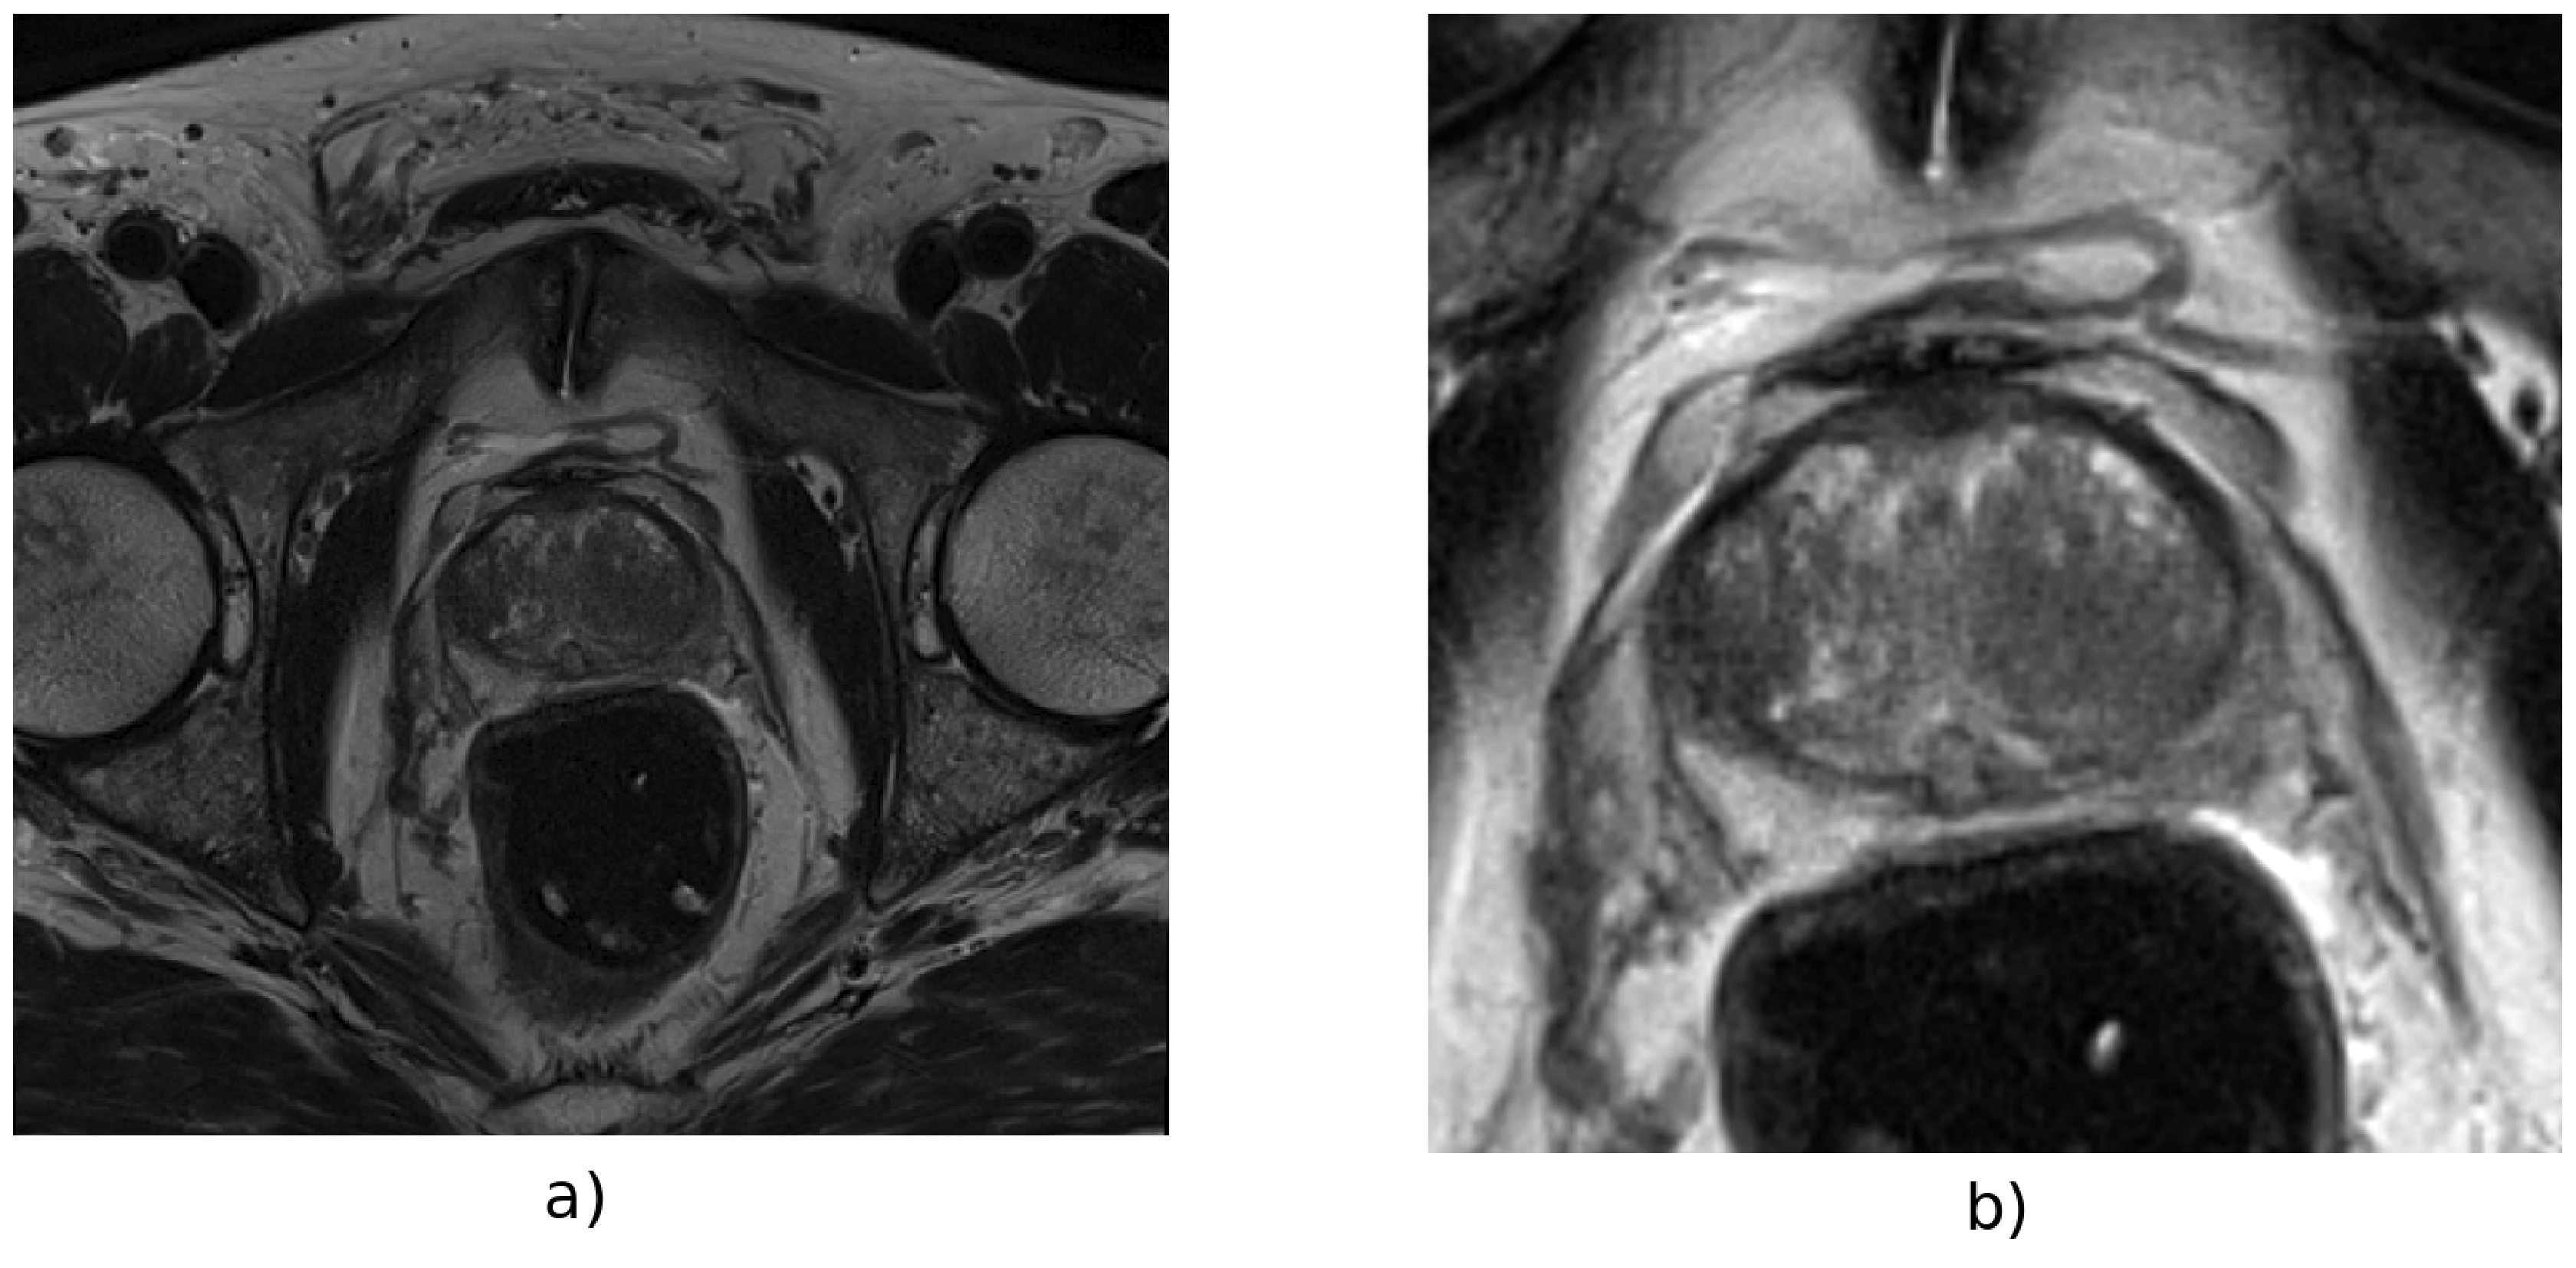
\includegraphics[totalheight=.25\textheight]{figures/Figure1.eps}
    \caption{The MRIs are preprocessed with bias correction, normalization, resampling, and cropped to a ROI to reduce the variability of sizes and intensities between magnets. In this example, \textbf{a)} is the original image and \textbf{b)} is the image after being processed.} 
    \label{fig_1}
\end{figure}

\begin{figure}[ht]
    \centering
    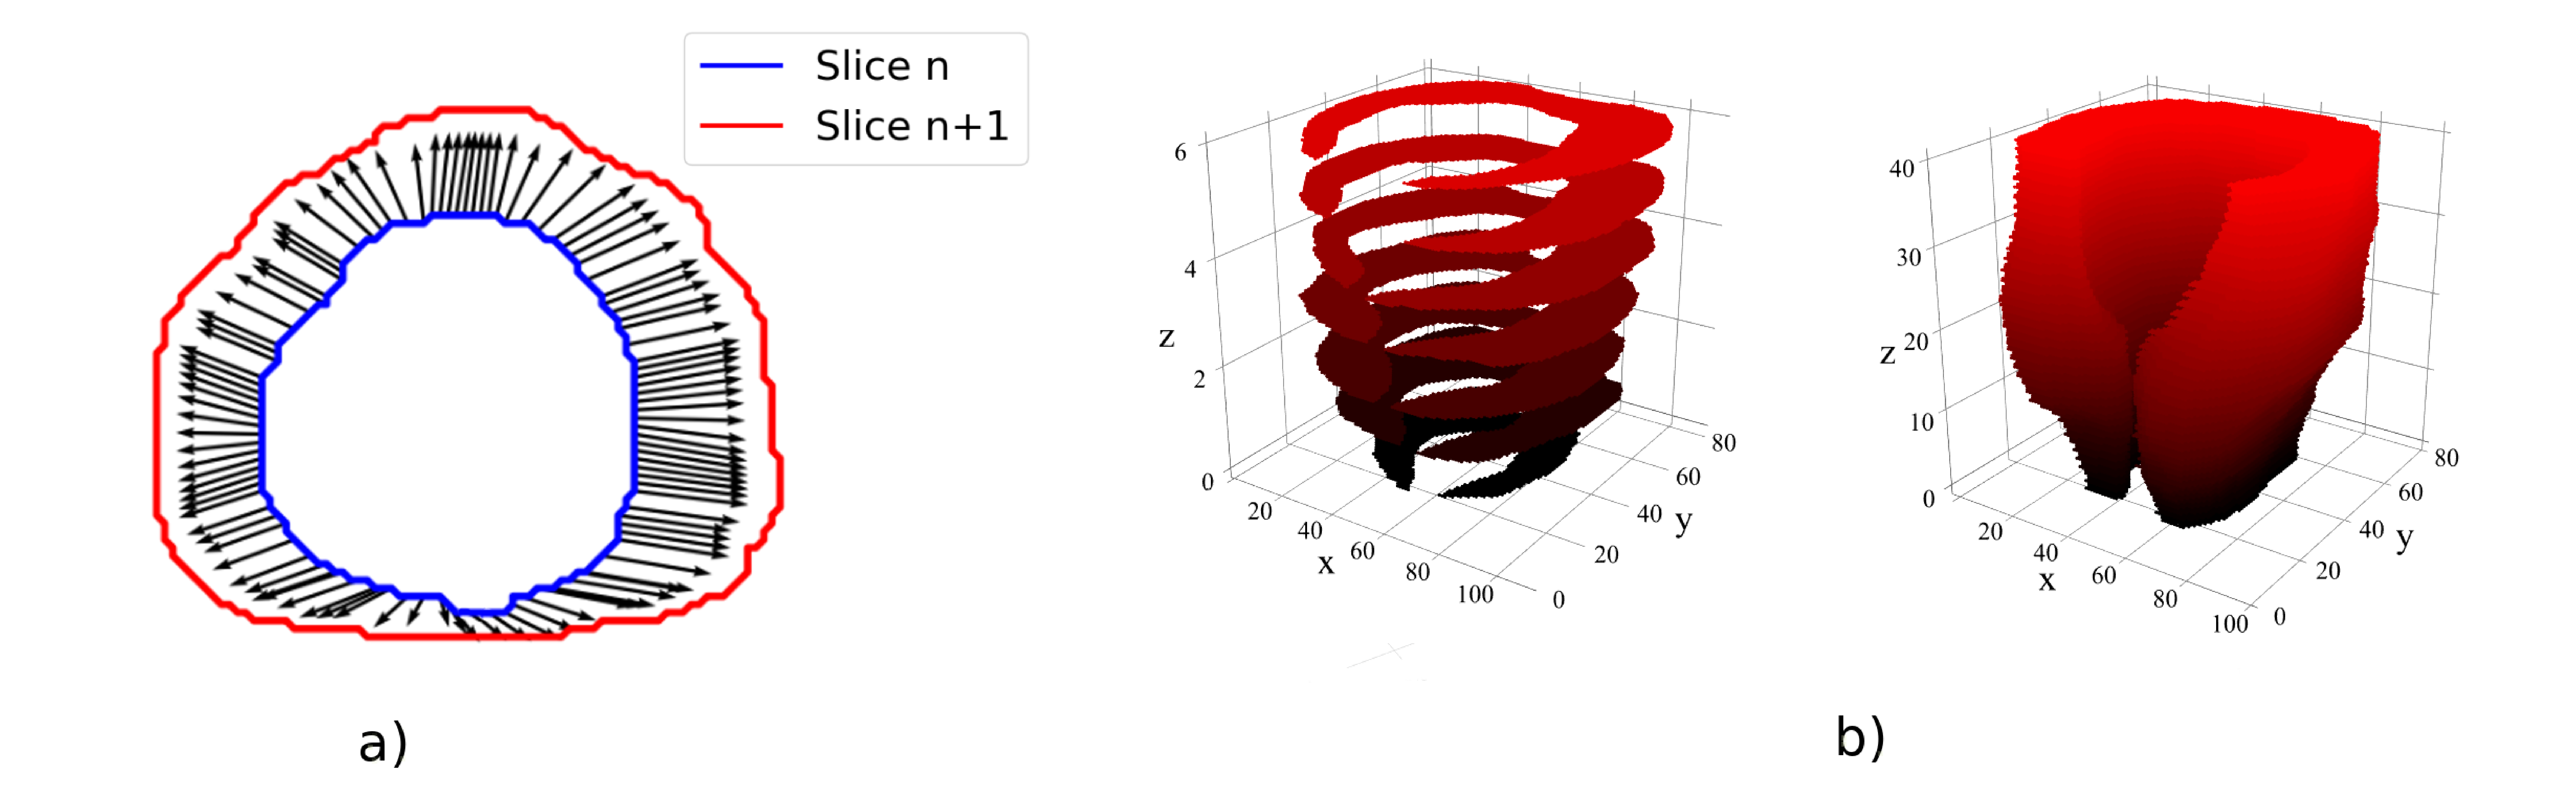
\includegraphics[totalheight=.21\textheight]{figures/Figure2.eps}
    \caption{Example of the proposed algorithm to increase the resolution of prostate and PZ contours. In \textbf{a)}, an example of the optical flow obtained between two prostate contours from adjacent horizontal planes. In \textbf{b)} on the left, original contours with 17 slices. On the right, interpolated contours with 68 slices.}
    \label{fig:fig_2}
\end{figure}

\begin{figure*}[ht]
    \centering
    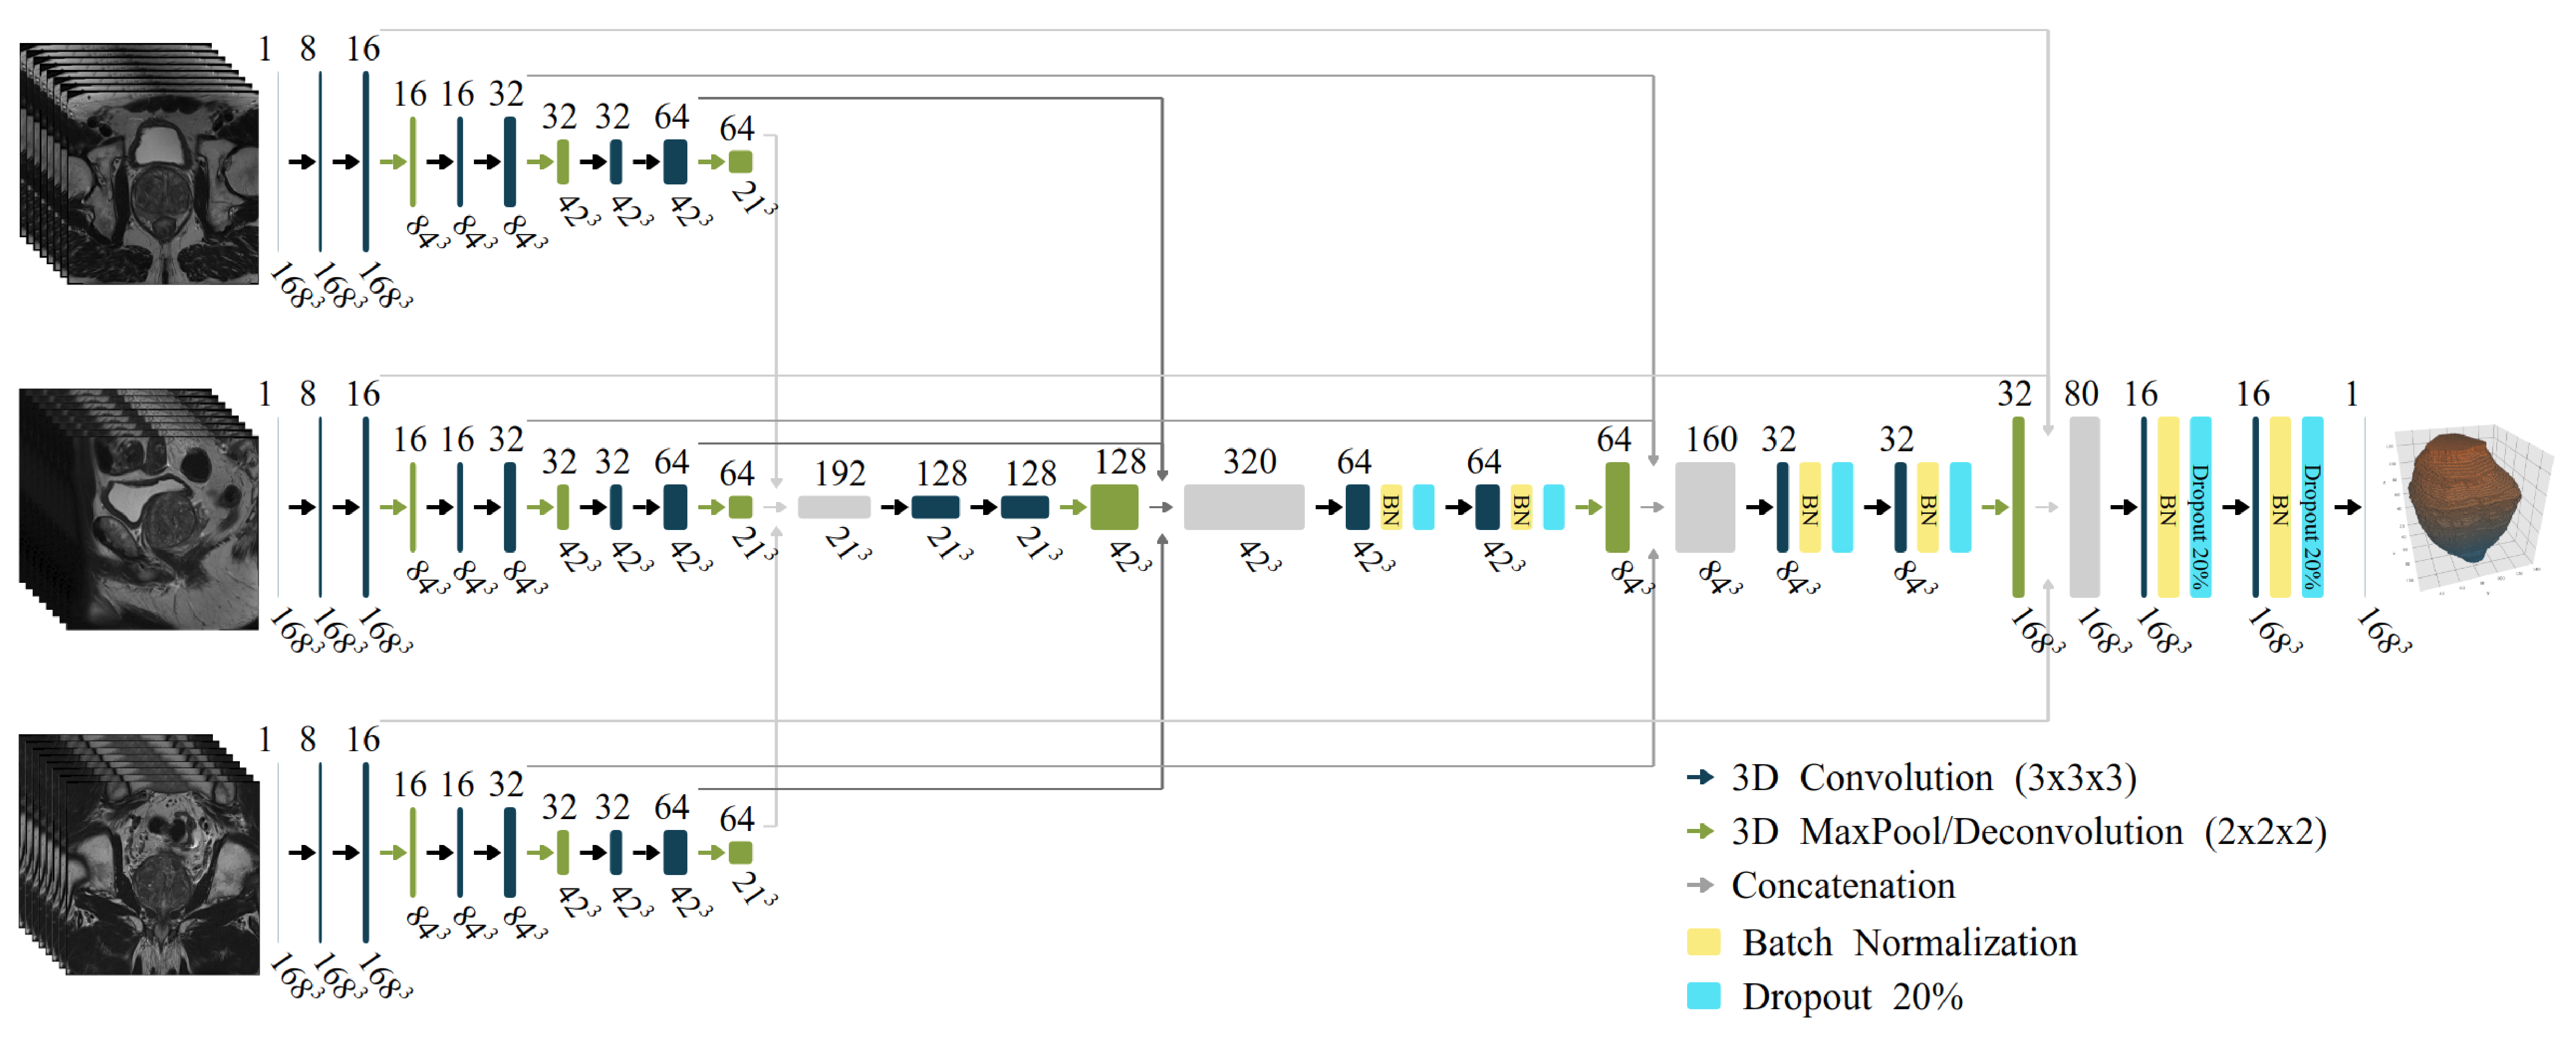
\includegraphics[totalheight=.282\textheight]{figures/Figure3.eps}
    \caption{Multistream 3D convolutional network architecture. The input of the network are three $168^3$ volumes from the MRI planes: axial, sagittal, and coronal. }
    \label{fig:fig_3}
\end{figure*}

\begin{figure}[ht]
    \centering
    \includegraphics[totalheight=.4\textheight]{figures/Figure4.eps}
    \caption{Prostate segmentation for the cases with the lowest, middle, and highest 3D DSC for the Siemens (up) and GE (down) datasets. These segmentation are obtained with the \emph{Combined} network model.  }
    \label{fig:resseg}
\end{figure} 

\begin{figure}[ht]
    \centering
    \includegraphics[totalheight=.4\textheight]{figures/Figure5.eps}
    \caption{Peripheral zone segmentation for the cases with the lowest, middle, and highest 3D DSC for the Siemens (up) and GE (down) datasets. These segmentation are obtained with the \emph{Combined} network model.  }
    \label{fig:ressegpz}
\end{figure} 
